
			\level{4}[BarChartDataImpl]{ApplicazioneAggiuntive::BarChartDataImpl}
			

		\IfFileExists{DefinizioneDiProdotto/Pics/ClassiAggiuntive/BarChartDataImpl.pdf}{
			\begin{figure}[H]
				\centering
				\includegraphics[scale=0.5]{DefinizioneDiProdotto/Pics/ClassiAggiuntive/BarChartDataImpl}
				\caption{BarChartDataImpl}
			\end{figure}
		}
	
			
			\begin{itemize}
			\item \textbf{Nome:} BarChartDataImpl
			\item \textbf{Tipo:} classe
			
		\item \textbf{Astratta:}
		no
			\item \textbf{Visibilità:} public
			\item \textbf{Descrizione:} Tale classe rappresenta i dati di un bar chart.
			\item \textbf{Attributi:}
				\begin{itemize}
				\setlength{\itemsep}{5pt}
				
					\item[\ding{111}] {--values : BarChart} \\ [1mm] Tale attributo rappresenta i valori del chart.
				\end{itemize}
		
			\item \textbf{Metodi:}
				\begin{itemize}
				\setlength{\itemsep}{5pt}
				
					\item[\ding{111}] {{+BarChartDataImpl(values : BarChart)}} \\ [1mm] Tale metodo è il costruttore di BarChartDataImpl. Esso ha come parametro i valori dei dati del chart.
					\item[\ding{111}] {{+getData() : BarChart}} \\ [1mm] Tale metodo ha il compito di ritornare i dati del chart.
					\item[\ding{111}] {{+setData(values : BarChart) : void}} \\ [1mm] Tale metodo ha il compito di impostare i dati del chart.
				\end{itemize}
		
			\end{itemize}
	
			\level{4}[BarChartElementInPlaceUpdate]{ApplicazioneAggiuntive::BarChartElementInPlaceUpdate}
			

		\IfFileExists{DefinizioneDiProdotto/Pics/ClassiAggiuntive/BarChartElementInPlaceUpdate.pdf}{
			\begin{figure}[H]
				\centering
				\includegraphics[scale=0.5]{DefinizioneDiProdotto/Pics/ClassiAggiuntive/BarChartElementInPlaceUpdate}
				\caption{BarChartElementInPlaceUpdate}
			\end{figure}
		}
	
			
			\begin{itemize}
			\item \textbf{Nome:} BarChartElementInPlaceUpdate
			\item \textbf{Tipo:} classe
			
		\item \textbf{Astratta:}
		no
			\item \textbf{Visibilità:} public
			\item \textbf{Descrizione:} Tale classe rappresenta un elemento di pacchetto di aggiornamento in place di un bar chart.
			\item \textbf{Attributi:}
				\begin{itemize}
				\setlength{\itemsep}{5pt}
				
					\item[\ding{111}] {--value : int} \\ [1mm] Tale attributo rappresenta i valori del dato aggiornato.
					\item[\ding{111}] {--xpos : int} \\ [1mm] Tale attributo rappresenta l'ordinata del dato da sostituire.
					\item[\ding{111}] {--ypos : int} \\ [1mm] Tale attributo rappresenta l'ascissa del dato da sostituire.
				\end{itemize}
		
			\item \textbf{Metodi:}
				\begin{itemize}
				\setlength{\itemsep}{5pt}
				
					\item[\ding{111}] {{+BarChartElementInPlaceUpdater(value : int, x : int, y : int) : void}} \\ [1mm] Tale metodo è il costruttore per create tale pacchetto di aggiornamento.
					\item[\ding{111}] {{+getData() : int}} \\ [1mm] Tale metodo ha il compito di ritornare il nuovo dato del pacchetto di aggiornamento.
					\item[\ding{111}] {{+getX() : int}} \\ [1mm] Tale metodo ha il compito di ritornare l'ascissa del dato da modificare.
					\item[\ding{111}] {{+getY() : int}} \\ [1mm] Tale metodo ha il compito di ritornare l'ordinata del dato da modificare.
				\end{itemize}
		
			\end{itemize}
	
			\level{4}[BarChartInPlaceUpdate]{ApplicazioneAggiuntive::BarChartInPlaceUpdate}
			

		\IfFileExists{DefinizioneDiProdotto/Pics/ClassiAggiuntive/BarChartInPlaceUpdate.pdf}{
			\begin{figure}[H]
				\centering
				\includegraphics[scale=0.5]{DefinizioneDiProdotto/Pics/ClassiAggiuntive/BarChartInPlaceUpdate}
				\caption{BarChartInPlaceUpdate}
			\end{figure}
		}
	
			
			\begin{itemize}
			\item \textbf{Nome:} BarChartInPlaceUpdate
			\item \textbf{Tipo:} classe
			
		\item \textbf{Astratta:}
		no
			\item \textbf{Visibilità:} public
			\item \textbf{Descrizione:} Tale classe rappresenta un pacchetto di aggiornamento in place di un bar chart.
			\item \textbf{Attributi:}
				\begin{itemize}
				\setlength{\itemsep}{5pt}
				
					\item[\ding{111}] {--values : ArrayList<BarChartElementInPlaceUpdater>} \\ [1mm] Tale attributo rappresenta i valori del dato aggiornato.
				\end{itemize}
		
			\item \textbf{Metodi:}
				\begin{itemize}
				\setlength{\itemsep}{5pt}
				
					\item[\ding{111}] {{+BarChartInPlaceUpdater(values : ArrayList<BarChartElementInPlaceUpdater>)}} \\ [1mm] Tale metodo è il costruttore per creare tale pacchetto di aggiornamento.
					\item[\ding{111}] {{+getData() : ArrayList<BarChartElementInPlaceUpdater>}} \\ [1mm] Tale metodo ha il compito di ritornare i dati del pacchetto di aggiornamento.
				\end{itemize}
		
			\end{itemize}
	
			\level{4}[BarChartSettingsImpl]{ApplicazioneAggiuntive::BarChartSettingsImpl}
			

		\IfFileExists{DefinizioneDiProdotto/Pics/ClassiAggiuntive/BarChartSettingsImpl.pdf}{
			\begin{figure}[H]
				\centering
				\includegraphics[scale=0.5]{DefinizioneDiProdotto/Pics/ClassiAggiuntive/BarChartSettingsImpl}
				\caption{BarChartSettingsImpl}
			\end{figure}
		}
	
			
			\begin{itemize}
			\item \textbf{Nome:} BarChartSettingsImpl
			\item \textbf{Tipo:} classe
			
		\item \textbf{Astratta:}
		no
			\item \textbf{Visibilità:} public
			\item \textbf{Descrizione:} Tale classe rappresenta le impostazioni di un bar chart.
			\item \textbf{Attributi:}
				\begin{itemize}
				\setlength{\itemsep}{5pt}
				
					\item[\ding{111}] {--settings : JSONObject} \\ [1mm] Tale attributo memorizza l'Oggetto JSON con le impostazioni del chart.
				\end{itemize}
		
			\item \textbf{Metodi:}
				\begin{itemize}
				\setlength{\itemsep}{5pt}
				
					\item[\ding{111}] {{+BarChartSettingsImpl(settings : JSONObject)}} \\ [1mm] Tale metodo è il costruttore della classe. Esso ha il compito di creare l'oggetto e di inizializzarne i campi.
					\item[\ding{111}] {{+getXAxisName() : String}} \\ [1mm] Tale metodo ha il compito di ritornare il nome del nome dell'asse delle ascisse.
					\item[\ding{111}] {{+getYAxisName() : String}} \\ [1mm] Tale metodo ha il compito di ritornare il nome del nome dell'asse delle ordinate.
					\item[\ding{111}] {{+getGridVisibility() : boolean}} \\ [1mm] Tale metodo ha il compito di ritornare un booleano che dica se la griglia è visualizzata o no.
					\item[\ding{111}] {{+getLegendPosition() : String}} \\ [1mm] Tale metodo ha il compito di ritornare la posizione della legenda.
					\item[\ding{111}] {{+getOrientation() : String}} \\ [1mm] Tale metodo ha il compito di ritornare l'orientamento del chart.
					\item[\ding{111}] {{+getTitle() : String}} \\ [1mm] Tale metodo ha il compito di ritornare il titolo del chart.
					\item[\ding{111}] {{+getDescription() : String}} \\ [1mm] Tale metodo ha il compito di ritornare la descrizione del chart.
					\item[\ding{111}] {{+getMaxValue() : String}} \\ [1mm] Tale metodo ha il compito di ritornare il numero massimo di valori consentiti nel chart.
					\item[\ding{111}] {{+getBarDataSetSpacing() : int}}
					\item[\ding{111}] {{+getBarValueSpacing() : int}}
				\end{itemize}
		
			\end{itemize}
	
			\level{4}[LineChartDataImpl]{ApplicazioneAggiuntive::LineChartDataImpl}
			

		\IfFileExists{DefinizioneDiProdotto/Pics/ClassiAggiuntive/LineChartDataImpl.pdf}{
			\begin{figure}[H]
				\centering
				\includegraphics[scale=0.5]{DefinizioneDiProdotto/Pics/ClassiAggiuntive/LineChartDataImpl}
				\caption{LineChartDataImpl}
			\end{figure}
		}
	
			
			\begin{itemize}
			\item \textbf{Nome:} LineChartDataImpl
			\item \textbf{Tipo:} classe
			
		\item \textbf{Astratta:}
		no
			\item \textbf{Visibilità:} public
			\item \textbf{Descrizione:} Tale classe rappresenta i dati di un line chart.
			\item \textbf{Attributi:}
				\begin{itemize}
				\setlength{\itemsep}{5pt}
				
					\item[\ding{111}] {--values : LineChart} \\ [1mm] Tale attributo rappresenta i valori del chart.
				\end{itemize}
		
			\item \textbf{Metodi:}
				\begin{itemize}
				\setlength{\itemsep}{5pt}
				
					\item[\ding{111}] {{+LineChartDataImpl(values : LineChart)}} \\ [1mm] Tale metodo è il costruttore di LineChartDataImpl. Esso ha come parametro i valori dei dati del chart.
					\item[\ding{111}] {{+getData() : LineChart}} \\ [1mm] Tale metodo ha il compito di ritornare i dati del chart.
					\item[\ding{111}] {{+setData(values : LineChart) : void}} \\ [1mm] Tale metodo ha il compito di impostare i dati del chart.
				\end{itemize}
		
			\end{itemize}
	
			\level{4}[LineChartElementInPlaceUpdate]{ApplicazioneAggiuntive::LineChartElementInPlaceUpdate}
			

		\IfFileExists{DefinizioneDiProdotto/Pics/ClassiAggiuntive/LineChartElementInPlaceUpdate.pdf}{
			\begin{figure}[H]
				\centering
				\includegraphics[scale=0.5]{DefinizioneDiProdotto/Pics/ClassiAggiuntive/LineChartElementInPlaceUpdate}
				\caption{LineChartElementInPlaceUpdate}
			\end{figure}
		}
	
			
			\begin{itemize}
			\item \textbf{Nome:} LineChartElementInPlaceUpdate
			\item \textbf{Tipo:} classe
			
		\item \textbf{Astratta:}
		no
			\item \textbf{Visibilità:} public
			\item \textbf{Descrizione:} Tale classe rappresenta un elemento di pacchetto di aggiornamento in place di un line chart.
			\item \textbf{Attributi:}
				\begin{itemize}
				\setlength{\itemsep}{5pt}
				
					\item[\ding{111}] {--value : int} \\ [1mm] Tale attributo rappresenta i valori del dato aggiornato.
					\item[\ding{111}] {--xpos : int} \\ [1mm] Tale attributo rappresenta l'ordinata del dato da sostituire.
					\item[\ding{111}] {--ypos : int} \\ [1mm] Tale attributo rappresenta l'ascissa del dato da sostituire.
				\end{itemize}
		
			\item \textbf{Metodi:}
				\begin{itemize}
				\setlength{\itemsep}{5pt}
				
					\item[\ding{111}] {{+LineChartElementInPlaceUpdater(value : int, x : int, y : int)}} \\ [1mm] Tale metodo è il costruttore per create tale pacchetto di aggiornamento.
					\item[\ding{111}] {{+getData() : int}} \\ [1mm] Tale metodo ha il compito di ritornare il nuovo dato del pacchetto di aggiornamento.
					\item[\ding{111}] {{+getX() : int}} \\ [1mm] Tale metodo ha il compito di ritornare l'ascissa del dato da modificare.
					\item[\ding{111}] {{+getY() : int}} \\ [1mm] Tale metodo ha il compito di ritornare l'ordinata del dato da modificare.
				\end{itemize}
		
			\end{itemize}
	
			\level{4}[LineChartElementStreamUpdate]{ApplicazioneAggiuntive::LineChartElementStreamUpdate}
			

		\IfFileExists{DefinizioneDiProdotto/Pics/ClassiAggiuntive/LineChartElementStreamUpdate.pdf}{
			\begin{figure}[H]
				\centering
				\includegraphics[scale=0.5]{DefinizioneDiProdotto/Pics/ClassiAggiuntive/LineChartElementStreamUpdate}
				\caption{LineChartElementStreamUpdate}
			\end{figure}
		}
	
			
			\begin{itemize}
			\item \textbf{Nome:} LineChartElementStreamUpdate
			\item \textbf{Tipo:} classe
			
		\item \textbf{Astratta:}
		no
			\item \textbf{Visibilità:} public
			\item \textbf{Descrizione:} Tale classe rappresenta un elemento di pacchetto di aggiornamento stream di un line chart.
			\item \textbf{Attributi:}
				\begin{itemize}
				\setlength{\itemsep}{5pt}
				
					\item[\ding{111}] {--label : String} \\ [1mm] Tale attributo rappresenta ivalore della nuova ettichetta da inserire nel chart.
					\item[\ding{111}] {--value : ArrayList<Integer>} \\ [1mm] Tale attributo rappresenta i valori del dato aggiornato.
				\end{itemize}
		
			\item \textbf{Metodi:}
				\begin{itemize}
				\setlength{\itemsep}{5pt}
				
					\item[\ding{111}] {{+LineChartElementStreamUpdater(label : String, value : ArrayList<Integer>)}} \\ [1mm] Tale metodo è il costruttore per create tale pacchetto di aggiornamento.
					\item[\ding{111}] {{+getData() : ArrayList<Integer>}} \\ [1mm] Tale metodo ha il compito di ritornare il nuovo dato del pacchetto di aggiornamento.
					\item[\ding{111}] {{+getLabel() : String}} \\ [1mm] Tale metodo ha il compito di ritornare il valore nella nuova etichetta.
				\end{itemize}
		
			\end{itemize}
	
			\level{4}[LineChartInPlaceUpdate]{ApplicazioneAggiuntive::LineChartInPlaceUpdate}
			

		\IfFileExists{DefinizioneDiProdotto/Pics/ClassiAggiuntive/LineChartInPlaceUpdate.pdf}{
			\begin{figure}[H]
				\centering
				\includegraphics[scale=0.5]{DefinizioneDiProdotto/Pics/ClassiAggiuntive/LineChartInPlaceUpdate}
				\caption{LineChartInPlaceUpdate}
			\end{figure}
		}
	
			
			\begin{itemize}
			\item \textbf{Nome:} LineChartInPlaceUpdate
			\item \textbf{Tipo:} classe
			
		\item \textbf{Astratta:}
		no
			\item \textbf{Visibilità:} public
			\item \textbf{Descrizione:} Tale classe rappresenta un pacchetto di aggiornamento in place di un line chart.
			\item \textbf{Attributi:}
				\begin{itemize}
				\setlength{\itemsep}{5pt}
				
					\item[\ding{111}] {--values : ArrayList<LineChartElementInPlaceUpdater>} \\ [1mm] Tale attributo rappresenta i valori del dato aggiornato.
				\end{itemize}
		
			\item \textbf{Metodi:}
				\begin{itemize}
				\setlength{\itemsep}{5pt}
				
					\item[\ding{111}] {{+LineChartInPlaceUpdater(values : ArrayList<LineChartElementInPlaceUpdater>)}} \\ [1mm] Tale metodo è il costruttore per creare tale pacchetto di aggiornamento.
					\item[\ding{111}] {{+getData() : ArrayList<LineChartElementInPlaceUpdater>}} \\ [1mm] Tale metodo ha il compito di ritornare i dati del pacchetto di aggiornamento.
				\end{itemize}
		
			\end{itemize}
	
			\level{4}[LineChartSettingsImpl]{ApplicazioneAggiuntive::LineChartSettingsImpl}
			

		\IfFileExists{DefinizioneDiProdotto/Pics/ClassiAggiuntive/LineChartSettingsImpl.pdf}{
			\begin{figure}[H]
				\centering
				\includegraphics[scale=0.5]{DefinizioneDiProdotto/Pics/ClassiAggiuntive/LineChartSettingsImpl}
				\caption{LineChartSettingsImpl}
			\end{figure}
		}
	
			
			\begin{itemize}
			\item \textbf{Nome:} LineChartSettingsImpl
			\item \textbf{Tipo:} classe
			
		\item \textbf{Astratta:}
		no
			\item \textbf{Visibilità:} public
			\item \textbf{Descrizione:} Tale classe rappresenta le impostazioni di un line chart.
			\item \textbf{Attributi:}
				\begin{itemize}
				\setlength{\itemsep}{5pt}
				
					\item[\ding{111}] {--settings : JSONObject} \\ [1mm] Tale attributo memorizza l'Oggetto JSON con le impostazioni del chart.
				\end{itemize}
		
			\item \textbf{Metodi:}
				\begin{itemize}
				\setlength{\itemsep}{5pt}
				
					\item[\ding{111}] {{+LineChartSettingsImpl(settings : JSONObject)}} \\ [1mm] Tale metodo è il costruttore della classe. Esso ha il compito di creare l'oggetto e di inizializzarne i campi.
					\item[\ding{111}] {{+getXAxisName() : String}} \\ [1mm] Tale metodo ha il compito di ritornare il nome del nome dell'asse delle ascisse.
					\item[\ding{111}] {{+getYAxisName() : String}} \\ [1mm] Tale metodo ha il compito di ritornare il nome del nome dell'asse delle ordinate.
					\item[\ding{111}] {{+getGridVisibility() : boolean}} \\ [1mm] Tale metodo ha il compito di ritornare un booleano che dica se la griglia è visualizzata o no.
					\item[\ding{111}] {{+getLegendPosition() : String}} \\ [1mm] Tale metodo ha il compito di ritornare la posizione della legenda.
					\item[\ding{111}] {{+getTitle() : String}} \\ [1mm] Tale metodo ha il compito di ritornare il titolo del chart.
					\item[\ding{111}] {{+getDescription() : String}} \\ [1mm] Tale metodo ha il compito di ritornare la descrizione del chart.
					\item[\ding{111}] {{+getMaxValue() : String}} \\ [1mm] Tale metodo ha il compito di ritornare il numero massimo di valori consentiti nel chart.
					\item[\ding{111}] {{+getDotRadius() : int}}
					\item[\ding{111}] {{+getCubicCurves() : boolean}}
				\end{itemize}
		
			\end{itemize}
	
			\level{4}[LineChartStreamUpdate]{ApplicazioneAggiuntive::LineChartStreamUpdate}
			

		\IfFileExists{DefinizioneDiProdotto/Pics/ClassiAggiuntive/LineChartStreamUpdate.pdf}{
			\begin{figure}[H]
				\centering
				\includegraphics[scale=0.5]{DefinizioneDiProdotto/Pics/ClassiAggiuntive/LineChartStreamUpdate}
				\caption{LineChartStreamUpdate}
			\end{figure}
		}
	
			
			\begin{itemize}
			\item \textbf{Nome:} LineChartStreamUpdate
			\item \textbf{Tipo:} classe
			
		\item \textbf{Astratta:}
		no
			\item \textbf{Visibilità:} public
			\item \textbf{Descrizione:} Tale classe rappresenta un pacchetto di aggiornamento stream di un line chart.
			\item \textbf{Attributi:}
				\begin{itemize}
				\setlength{\itemsep}{5pt}
				
					\item[\ding{111}] {--values : ArrayList<LineChartElementStreamUpdater>} \\ [1mm] Tale attributo rappresenta i valori del dato aggiornato.
				\end{itemize}
		
			\item \textbf{Metodi:}
				\begin{itemize}
				\setlength{\itemsep}{5pt}
				
					\item[\ding{111}] {{+LineChartStreamUpdater(values : ArrayList<LineChartElementStreamUpdater>)}} \\ [1mm] Tale metodo è il costruttore per creare tale pacchetto di aggiornamento.
					\item[\ding{111}] {{+getData() : ArrayList<LineChartElementStreamUpdater>}} \\ [1mm] Tale metodo ha il compito di ritornare i dati del pacchetto di aggiornamento.
				\end{itemize}
		
			\end{itemize}
	
			\level{4}[MapChartDataImpl]{ApplicazioneAggiuntive::MapChartDataImpl}
			

		\IfFileExists{DefinizioneDiProdotto/Pics/ClassiAggiuntive/MapChartDataImpl.pdf}{
			\begin{figure}[H]
				\centering
				\includegraphics[scale=0.5]{DefinizioneDiProdotto/Pics/ClassiAggiuntive/MapChartDataImpl}
				\caption{MapChartDataImpl}
			\end{figure}
		}
	
			
			\begin{itemize}
			\item \textbf{Nome:} MapChartDataImpl
			\item \textbf{Tipo:} classe
			
		\item \textbf{Astratta:}
		no
			\item \textbf{Visibilità:} public
			\item \textbf{Descrizione:} Tale classe rappresenta i dati di un map chart.
			\item \textbf{Attributi:}
				\begin{itemize}
				\setlength{\itemsep}{5pt}
				
					\item[\ding{111}] {--values : ArrayList<MapSet>} \\ [1mm] Tale attributo rappresenta i valori del chart.
				\end{itemize}
		
			\item \textbf{Metodi:}
				\begin{itemize}
				\setlength{\itemsep}{5pt}
				
					\item[\ding{111}] {{+MapChartImpl(values : ArrayList<MapSet>)}} \\ [1mm] Tale metodo è il costruttore di MapChartDataImpl. Esso ha come parametro i valori dei dati del chart.
					\item[\ding{111}] {{+getData() : ArrayList<MapSet>}} \\ [1mm] Tale metodo ha il compito di ritornare i dati del chart.
					\item[\ding{111}] {{+setData(values : ArrayList<MapSet>) : void}} \\ [1mm] Tale metodo ha il compito di impostare i dati del chart.
				\end{itemize}
		
			\end{itemize}
	
			\level{4}[MapChartDeleteUpdate]{ApplicazioneAggiuntive::MapChartDeleteUpdate}
			

		\IfFileExists{DefinizioneDiProdotto/Pics/ClassiAggiuntive/MapChartDeleteUpdate.pdf}{
			\begin{figure}[H]
				\centering
				\includegraphics[scale=0.5]{DefinizioneDiProdotto/Pics/ClassiAggiuntive/MapChartDeleteUpdate}
				\caption{MapChartDeleteUpdate}
			\end{figure}
		}
	
			
			\begin{itemize}
			\item \textbf{Nome:} MapChartDeleteUpdate
			\item \textbf{Tipo:} classe
			
		\item \textbf{Astratta:}
		no
			\item \textbf{Visibilità:} public
			\item \textbf{Descrizione:} Tale classe rappresenta un pacchetto di eliminazione di un map chart.
			\item \textbf{Attributi:}
				\begin{itemize}
				\setlength{\itemsep}{5pt}
				
					\item[\ding{111}] {--values : ArrayList<ArrayList<MapChartElementDeleteUpdate>} \\ [1mm] Tale attributo rappresenta i valori del dato aggiornato.
				\end{itemize}
		
			\item \textbf{Metodi:}
				\begin{itemize}
				\setlength{\itemsep}{5pt}
				
					\item[\ding{111}] {{+MapChartDeleteUpdate(values : ArrayList<ArrayList<MapChartElementDeleteUpdate>)}} \\ [1mm] Tale metodo è il costruttore per create tale pacchetto di aggiornamento.
					\item[\ding{111}] {{+getData() : ArrayList<ArrayList<MapChartElementDeleteUpdate>}} \\ [1mm] Tale metodo ha il compito di ritornare i nuovi dati del pacchetto di aggiornamento.
				\end{itemize}
		
			\end{itemize}
	
			\level{4}[MapChartElementDeleteUpdate]{ApplicazioneAggiuntive::MapChartElementDeleteUpdate}
			

		\IfFileExists{DefinizioneDiProdotto/Pics/ClassiAggiuntive/MapChartElementDeleteUpdate.pdf}{
			\begin{figure}[H]
				\centering
				\includegraphics[scale=0.5]{DefinizioneDiProdotto/Pics/ClassiAggiuntive/MapChartElementDeleteUpdate}
				\caption{MapChartElementDeleteUpdate}
			\end{figure}
		}
	
			
			\begin{itemize}
			\item \textbf{Nome:} MapChartElementDeleteUpdate
			\item \textbf{Tipo:} classe
			
		\item \textbf{Astratta:}
		no
			\item \textbf{Visibilità:} public
			\item \textbf{Attributi:}
				\begin{itemize}
				\setlength{\itemsep}{5pt}
				
					\item[\ding{111}] {--value : MapPoint} \\ [1mm] Rappresenta un punto da aggiungere in stream alla mappa.
					\item[\ding{111}] {--series : int} \\ [1mm] Indica a quale serie di valori tale punto deve esser aggiunto.
					\item[\ding{111}] {--index : int} \\ [1mm] Indica a quale indice della serie di valori del punto da rimuovere.
				\end{itemize}
		
			\item \textbf{Metodi:}
				\begin{itemize}
				\setlength{\itemsep}{5pt}
				
					\item[\ding{111}] {{+getData() : MapPoint}} \\ [1mm] Tale metodo ritorna il valore dell'elemento di aggiornamento.
					\item[\ding{111}] {{+getSeries() : int}} \\ [1mm] Tale metodo ritorna in numero della serie al quale si riperisce l'elemento di aggiornamento.
					\item[\ding{111}] {{+getIndex() : int}} \\ [1mm] Tale metodo ritorna in numero dell'indice della serie al quale si riperisce l'elemento di aggiornamento.
					\item[\ding{111}] {{+MapChartElementDeleteUpdate(value : MapPoint, series : int, index : int)}} \\ [1mm] Tale metodo rappresenta il costruttore dell'elemento di aggiornamento. Esso Richiede 3 parametri: il numero della serie e l'indice al quale si riferisce tale aggiornamento ed il valore del punto dell'aggiornamento.
				\end{itemize}
		
			\end{itemize}
	
			\level{4}[MapChartElementInPlaceUpdate]{ApplicazioneAggiuntive::MapChartElementInPlaceUpdate}
			

		\IfFileExists{DefinizioneDiProdotto/Pics/ClassiAggiuntive/MapChartElementInPlaceUpdate.pdf}{
			\begin{figure}[H]
				\centering
				\includegraphics[scale=0.5]{DefinizioneDiProdotto/Pics/ClassiAggiuntive/MapChartElementInPlaceUpdate}
				\caption{MapChartElementInPlaceUpdate}
			\end{figure}
		}
	
			
			\begin{itemize}
			\item \textbf{Nome:} MapChartElementInPlaceUpdate
			\item \textbf{Tipo:} classe
			
		\item \textbf{Astratta:}
		no
			\item \textbf{Visibilità:} public
			\item \textbf{Descrizione:} Tale classe rappresenta un elemento di pacchetto di aggiornamento in place di un map chart.
			\item \textbf{Attributi:}
				\begin{itemize}
				\setlength{\itemsep}{5pt}
				
					\item[\ding{111}] {--value : MapPoint} \\ [1mm] Tale attributo rappresenta i valori del dato aggiornato.
					\item[\ding{111}] {--x : int} \\ [1mm] Tale attributo rappresenta l'ordinata nella mappa del dato da sostituire.
					\item[\ding{111}] {--y : int} \\ [1mm] Tale attributo rappresenta l'ascissa nella mappa del dato da sostituire.
				\end{itemize}
		
			\item \textbf{Metodi:}
				\begin{itemize}
				\setlength{\itemsep}{5pt}
				
					\item[\ding{111}] {{+MapChartElementInPlaceUpdate(value : MapPoint, x : int, y : int)}} \\ [1mm] Tale metodo è un costruttore per create tale pacchetto di aggiornamento.
					\item[\ding{111}] {{+getData() : MapPoint}} \\ [1mm] Tale metodo ha il compito di ritornare i nuovi dati del pacchetto di aggiornamento.
					\item[\ding{111}] {{+getX() : double}} \\ [1mm] Tale metodo ha il compito di ritornare la posizione nel mapchart del punto da modificare.
					\item[\ding{111}] {{+getY() : double}} \\ [1mm] Tale metodo ha il compito di ritornare la posizione nel mapchart del punto da modificare.
					\item[\ding{111}] {{+getId() : String}} \\ [1mm] Tale metodo ha il compito di ritornare l'id del punto da modificare.
				\end{itemize}
		
			\end{itemize}
	
			\level{4}[MapChartElementStreamUpdate]{ApplicazioneAggiuntive::MapChartElementStreamUpdate}
			

		\IfFileExists{DefinizioneDiProdotto/Pics/ClassiAggiuntive/MapChartElementStreamUpdate.pdf}{
			\begin{figure}[H]
				\centering
				\includegraphics[scale=0.5]{DefinizioneDiProdotto/Pics/ClassiAggiuntive/MapChartElementStreamUpdate}
				\caption{MapChartElementStreamUpdate}
			\end{figure}
		}
	
			
			\begin{itemize}
			\item \textbf{Nome:} MapChartElementStreamUpdate
			\item \textbf{Tipo:} classe
			
		\item \textbf{Astratta:}
		no
			\item \textbf{Visibilità:} public
			\item \textbf{Attributi:}
				\begin{itemize}
				\setlength{\itemsep}{5pt}
				
					\item[\ding{111}] {--value : MapPoint} \\ [1mm] Rappresenta un punto da aggiungere in stream alla mappa.
					\item[\ding{111}] {--series : int} \\ [1mm] Indica a quale serie di valori tale punto deve esser aggiunto.
				\end{itemize}
		
			\item \textbf{Metodi:}
				\begin{itemize}
				\setlength{\itemsep}{5pt}
				
					\item[\ding{111}] {{+MapChartElementStreamUpdate(series : int, value : MapPoint)}} \\ [1mm] Tale metodo rappresenta il costruttore dell'elemento di aggiornamento. Esso Richiede 2 parametri: il numero della serie al quale si riferisce tale aggiornamento ed il valore del punto dell'aggiornamento.
					\item[\ding{111}] {{+getData() : MapPoint}} \\ [1mm] Tale metodo ritorna il valore dell'elemento di aggiornamento.
					\item[\ding{111}] {{+getSeries() : int}} \\ [1mm] Tale metodo ritorna in numero della serie al quale si riperisce l'elemento di aggiornamento.
				\end{itemize}
		
			\end{itemize}
	
			\level{4}[MapChartInPlaceUpdate]{ApplicazioneAggiuntive::MapChartInPlaceUpdate}
			

		\IfFileExists{DefinizioneDiProdotto/Pics/ClassiAggiuntive/MapChartInPlaceUpdate.pdf}{
			\begin{figure}[H]
				\centering
				\includegraphics[scale=0.5]{DefinizioneDiProdotto/Pics/ClassiAggiuntive/MapChartInPlaceUpdate}
				\caption{MapChartInPlaceUpdate}
			\end{figure}
		}
	
			
			\begin{itemize}
			\item \textbf{Nome:} MapChartInPlaceUpdate
			\item \textbf{Tipo:} classe
			
		\item \textbf{Astratta:}
		no
			\item \textbf{Visibilità:} public
			\item \textbf{Descrizione:} Tale classe rappresenta un pacchetto di aggiornamento in place di un map chart.
			\item \textbf{Attributi:}
				\begin{itemize}
				\setlength{\itemsep}{5pt}
				
					\item[\ding{111}] {--values : ArrayList<MapChartElementInPlaceUpdate>} \\ [1mm] Tale attributo rappresenta i valori del dato aggiornato.
				\end{itemize}
		
			\item \textbf{Metodi:}
				\begin{itemize}
				\setlength{\itemsep}{5pt}
				
					\item[\ding{111}] {{+MapChartInPlaceUpdate(values : ArrayList<MapChartElementInPlaceUpdate>)}} \\ [1mm] Tale metodo è un costruttore per creare tale pacchetto di aggiornamento.
					\item[\ding{111}] {{+getData() : ArrayList<MapChartElementInPlaceUpdate>}} \\ [1mm] Tale metodo ha il compito di ritornare i nuovi dati del pacchetto di aggiornamento.
				\end{itemize}
		
			\end{itemize}
	
			\level{4}[MapChartMovieUpdate]{ApplicazioneAggiuntive::MapChartMovieUpdate}
			

		\IfFileExists{DefinizioneDiProdotto/Pics/ClassiAggiuntive/MapChartMovieUpdate.pdf}{
			\begin{figure}[H]
				\centering
				\includegraphics[scale=0.5]{DefinizioneDiProdotto/Pics/ClassiAggiuntive/MapChartMovieUpdate}
				\caption{MapChartMovieUpdate}
			\end{figure}
		}
	
			
			\begin{itemize}
			\item \textbf{Nome:} MapChartMovieUpdate
			\item \textbf{Tipo:} classe
			
		\item \textbf{Astratta:}
		no
			\item \textbf{Visibilità:} public
			\item \textbf{Descrizione:} Tale classe rappresenta un pacchetto di aggiornamento movie di un map chart.
			\item \textbf{Attributi:}
				\begin{itemize}
				\setlength{\itemsep}{5pt}
				
					\item[\ding{111}] {--inplace : MapChartInPlaceUpdate} \\ [1mm] Tale metodo ha il compito di memorizzare il pacchetto dell'aggiornamento InPlace sul chart.
					\item[\ding{111}] {--stream : MapChartStreamUpdate} \\ [1mm] Tale metodo ha il compito di memorizzare il pacchetto dell'aggiornamento Stream sul chart.
					\item[\ding{111}] {--delete : MapChartDeleteUpdate} \\ [1mm] Tale metodo ha il compito di memorizzare il pacchetto con i dati da eliminare dal chart.
				\end{itemize}
		
			\item \textbf{Metodi:}
				\begin{itemize}
				\setlength{\itemsep}{5pt}
				
					\item[\ding{111}] {{+MapChartMovieUpdate(inplace : MapChartInPlaceUpdate, stream : MapChartStreamUpdate, delete : MapChartDeleteUpdate)}} \\ [1mm] Tale metodo è il costruttore per create tale pacchetto di aggiornamento.
					\item[\ding{111}] {{+getInPlaceData() : MapChartInPlaceUpdate}} \\ [1mm] Tale metodo ha il compito di ritornare il pacchetto dell'aggiornamento InPlace sul chart.
					\item[\ding{111}] {{+getStreamData() : MapChartStreamUpdate}} \\ [1mm] Tale metodo ha il compito di ritornare il pacchetto dell'aggiornamento Stream sul chart.
					\item[\ding{111}] {{+getDeleteData() : MapChartDeleteUpdate}} \\ [1mm] Tale metodo ha il compito di ritornare il pacchetto con i dati da eliminare dal chart.
				\end{itemize}
		
			\end{itemize}
	
			\level{4}[MapChartSettingsImpl]{ApplicazioneAggiuntive::MapChartSettingsImpl}
			

		\IfFileExists{DefinizioneDiProdotto/Pics/ClassiAggiuntive/MapChartSettingsImpl.pdf}{
			\begin{figure}[H]
				\centering
				\includegraphics[scale=0.5]{DefinizioneDiProdotto/Pics/ClassiAggiuntive/MapChartSettingsImpl}
				\caption{MapChartSettingsImpl}
			\end{figure}
		}
	
			
			\begin{itemize}
			\item \textbf{Nome:} MapChartSettingsImpl
			\item \textbf{Tipo:} classe
			
		\item \textbf{Astratta:}
		no
			\item \textbf{Visibilità:} public
			\item \textbf{Descrizione:} Tale classe rappresenta le impostazioni di un map chart.
			\item \textbf{Attributi:}
				\begin{itemize}
				\setlength{\itemsep}{5pt}
				
					\item[\ding{111}] {--settings : JSONObject} \\ [1mm] Tale attributo memorizza l'Oggetto JSON con le impostazioni del chart.
				\end{itemize}
		
			\item \textbf{Metodi:}
				\begin{itemize}
				\setlength{\itemsep}{5pt}
				
					\item[\ding{111}] {{+MapChartSettingsImpl(settings : JSONObject)}} \\ [1mm] Tale metodo è il costruttore della classe. Esso ha il compito di creare l'oggetto e di inizializzarne i campi.
					\item[\ding{111}] {{+getXCameraCoordinate() : double}} \\ [1mm] Tale metodo ha il compito di ritornare le ascisse della posizione della camera nel map chart.
					\item[\ding{111}] {{+getYCameraCoordinate() : double}} \\ [1mm] Tale metodo ha il compito di ritornare le ordinate della posizione della camera nel map chart.
					\item[\ding{111}] {{+getCameraZoomHeight() : int}} \\ [1mm] Tale metodo ha il compito di ritornare l'altezza della camera nel map chart.
					\item[\ding{111}] {{+getTitle() : String}} \\ [1mm] Tale metodo ha il compito di ritornare il titolo del chart.
					\item[\ding{111}] {{+getDescription() : String}} \\ [1mm] Tale metodo ha il compito di ritornare la descrizione del chart.
					\item[\ding{111}] {{+getMaxValue() : String}} \\ [1mm] Tale metodo ha il compito di ritornare il numero massimo di valori consentiti nel chart.
				\end{itemize}
		
			\end{itemize}
	
			\level{4}[MapChartStreamUpdate]{ApplicazioneAggiuntive::MapChartStreamUpdate}
			

		\IfFileExists{DefinizioneDiProdotto/Pics/ClassiAggiuntive/MapChartStreamUpdate.pdf}{
			\begin{figure}[H]
				\centering
				\includegraphics[scale=0.5]{DefinizioneDiProdotto/Pics/ClassiAggiuntive/MapChartStreamUpdate}
				\caption{MapChartStreamUpdate}
			\end{figure}
		}
	
			
			\begin{itemize}
			\item \textbf{Nome:} MapChartStreamUpdate
			\item \textbf{Tipo:} classe
			
		\item \textbf{Astratta:}
		no
			\item \textbf{Visibilità:} public
			\item \textbf{Descrizione:} Tale classe rappresenta un pacchetto di aggiornamento stream di un map chart.
			\item \textbf{Attributi:}
				\begin{itemize}
				\setlength{\itemsep}{5pt}
				
					\item[\ding{111}] {--values : ArrayList<MapChartElementStreamUpdate>} \\ [1mm] Tale attributo rappresenta i valori del dato aggiornato.
				\end{itemize}
		
			\item \textbf{Metodi:}
				\begin{itemize}
				\setlength{\itemsep}{5pt}
				
					\item[\ding{111}] {{+MapChartStreamUpdate(values : ArrayList<MapChartElementStreamUpdate>)}} \\ [1mm] Tale metodo è il costruttore per create tale pacchetto di aggiornamento.
					\item[\ding{111}] {{+getData() : ArrayList<MapChartElementStreamUpdate>}} \\ [1mm] Tale metodo ha il compito di ritornare i nuovi dati del pacchetto di aggiornamento.
				\end{itemize}
		
			\end{itemize}
	
			\level{4}[MapPoint]{ApplicazioneAggiuntive::MapPoint}
			

		\IfFileExists{DefinizioneDiProdotto/Pics/ClassiAggiuntive/MapPoint.pdf}{
			\begin{figure}[H]
				\centering
				\includegraphics[scale=0.5]{DefinizioneDiProdotto/Pics/ClassiAggiuntive/MapPoint}
				\caption{MapPoint}
			\end{figure}
		}
	
			
			\begin{itemize}
			\item \textbf{Nome:} MapPoint
			\item \textbf{Tipo:} classe
			
		\item \textbf{Astratta:}
		no
			\item \textbf{Visibilità:} public
			\item \textbf{Descrizione:} Tale classe rappresenta i dati di un punto di un map chart.
			\item \textbf{Attributi:}
				\begin{itemize}
				\setlength{\itemsep}{5pt}
				
					\item[\ding{111}] {--latitude : double} \\ [1mm] Tale attributo rappresenta la latitudine di un punto del map chart.
					\item[\ding{111}] {--longitude : double} \\ [1mm] Tale attributo rappresenta la longitudine di un punto del map chart.
					\item[\ding{111}] {--id : String} \\ [1mm] Tale attributo rappresenta l'id di un punto del map chart.
				\end{itemize}
		
			\item \textbf{Metodi:}
				\begin{itemize}
				\setlength{\itemsep}{5pt}
				
					\item[\ding{111}] {{+MapPoint(lat : double, long : double, id : String)}} \\ [1mm] Tale metodo è il costruttore di MapPoint. Esso ha come parametri i valori di una coordinata geografica e l'id di questo.
					\item[\ding{111}] {{+getLongitude() : double}} \\ [1mm] Tale metodo ha il compito di ritornare la longitudine del punto.
					\item[\ding{111}] {{+getLatitude() : double}} \\ [1mm] Tale metodo ha il compito di ritornare la latitudine del punto.
					\item[\ding{111}] {{+getId() : String}} \\ [1mm] Tale metodo ha il compito di ritornare l'id del punto.
					\item[\ding{111}] {{+setLongitude(long : double) : void}} \\ [1mm] Tale metodo ha il compito di impostare la longitudine del punto.
					\item[\ding{111}] {{+setLatitude(lat : double) : void}} \\ [1mm] Tale metodo ha il compito di impostare la latitudine del punto.
				\end{itemize}
		
			\end{itemize}
	
			\level{4}[MapSet]{ApplicazioneAggiuntive::MapSet}
			

		\IfFileExists{DefinizioneDiProdotto/Pics/ClassiAggiuntive/MapSet.pdf}{
			\begin{figure}[H]
				\centering
				\includegraphics[scale=0.5]{DefinizioneDiProdotto/Pics/ClassiAggiuntive/MapSet}
				\caption{MapSet}
			\end{figure}
		}
	
			
			\begin{itemize}
			\item \textbf{Nome:} MapSet
			\item \textbf{Tipo:} classe
			
		\item \textbf{Astratta:}
		no
			\item \textbf{Visibilità:} public
			\item \textbf{Descrizione:} Tale classe rappresenta i dati di un set di un map chart.
			\item \textbf{Attributi:}
				\begin{itemize}
				\setlength{\itemsep}{5pt}
				
					\item[\ding{111}] {--values : ArrayList<MapPoint>} \\ [1mm] Tale attributo rappresenta i valori di una serie del map chart.
				\end{itemize}
		
			\item \textbf{Metodi:}
				\begin{itemize}
				\setlength{\itemsep}{5pt}
				
					\item[\ding{111}] {{+MapSet(values : ArrayList<MapPoint>)}} \\ [1mm] Tale metodo è il costruttore di MapSet. Esso ha come parametro i valori dei dati della serie di un mapchart.
					\item[\ding{111}] {{+getData() : ArrayList<MapPoint>}} \\ [1mm] Tale metodo ha il compito di ritornare i dati della serie.
					\item[\ding{111}] {{+setData(values : ArrayList<MapPoint>) : void}} \\ [1mm] Tale metodo ha il compito di impostare i dati della serie.
				\end{itemize}
		
			\end{itemize}
	
			\level{4}[TableCell]{ApplicazioneAggiuntive::TableCell}
			

		\IfFileExists{DefinizioneDiProdotto/Pics/ClassiAggiuntive/TableCell.pdf}{
			\begin{figure}[H]
				\centering
				\includegraphics[scale=0.5]{DefinizioneDiProdotto/Pics/ClassiAggiuntive/TableCell}
				\caption{TableCell}
			\end{figure}
		}
	
			
			\begin{itemize}
			\item \textbf{Nome:} TableCell
			\item \textbf{Tipo:} classe
			
		\item \textbf{Astratta:}
		no
			\item \textbf{Visibilità:} public
			\item \textbf{Descrizione:} Tale classe rappresenta i dati di una cella di una table.
			\item \textbf{Attributi:}
				\begin{itemize}
				\setlength{\itemsep}{5pt}
				
					\item[\ding{111}] {--fontColor : String} \\ [1mm] Tale attributo rappresenta il colore del testo di una cella della table.
					\item[\ding{111}] {--bgColor : String} \\ [1mm] Tale attributo rappresenta il colore di sfondo di una cella della table.
					\item[\ding{111}] {--value : String} \\ [1mm] Tale attributo rappresenta il valore di una cella della table.
				\end{itemize}
		
			\item \textbf{Metodi:}
				\begin{itemize}
				\setlength{\itemsep}{5pt}
				
					\item[\ding{111}] {{+TableCell(value : String, fontColor : String, bgColor : String)}} \\ [1mm] Tale metodo è il costruttore di TableRow. Esso ha come parametro i valori dei dati delle celle della riga della tabella.
					\item[\ding{111}] {{+getData() : String}} \\ [1mm] Tale metodo ha il compito di ritornare i dati della cella.
					\item[\ding{111}] {{+getBgColor() : String}} \\ [1mm] Tale metodo ha il compito di ritornare il colore di sfondo della cella.
					\item[\ding{111}] {{+getFontColor() : String}} \\ [1mm] Tale metodo ha il compito di ritornare il colore di testo della cella.
					\item[\ding{111}] {{+setData(value : String) : void}} \\ [1mm] Tale metodo ha il compito di impostare i dati della cella.
					\item[\ding{111}] {{+setBgColor(color : String) : void}} \\ [1mm] Tale metodo ha il compito di impostare il colore di sfondo della cella.
					\item[\ding{111}] {{+setFontColor(color : String) : void}} \\ [1mm] Tale metodo ha il compito di impostare il colore di sfondo della cella.
				\end{itemize}
		
			\end{itemize}
	
			\level{4}[TableCellInPlaceUpdate]{ApplicazioneAggiuntive::TableCellInPlaceUpdate}
			

		\IfFileExists{DefinizioneDiProdotto/Pics/ClassiAggiuntive/TableCellInPlaceUpdate.pdf}{
			\begin{figure}[H]
				\centering
				\includegraphics[scale=0.5]{DefinizioneDiProdotto/Pics/ClassiAggiuntive/TableCellInPlaceUpdate}
				\caption{TableCellInPlaceUpdate}
			\end{figure}
		}
	
			
			\begin{itemize}
			\item \textbf{Nome:} TableCellInPlaceUpdate
			\item \textbf{Tipo:} classe
			
		\item \textbf{Astratta:}
		no
			\item \textbf{Visibilità:} public
			\item \textbf{Descrizione:} Tale classe rappresenta un elemento di pacchetto di aggiornamento in place di una table.
			\item \textbf{Attributi:}
				\begin{itemize}
				\setlength{\itemsep}{5pt}
				
					\item[\ding{111}] {--xpos : int} \\ [1mm] Tale attributo rappresenta l'ordinata del dato da sostituire.
					\item[\ding{111}] {--ypos : int} \\ [1mm] Tale attributo rappresenta l'ascissa del dato da sostituire.
					\item[\ding{111}] {--value : String} \\ [1mm] Tale attributo memorizza il nuovo valore da inserire nel chart.
				\end{itemize}
		
			\item \textbf{Metodi:}
				\begin{itemize}
				\setlength{\itemsep}{5pt}
				
					\item[\ding{111}] {{+TableCellInPlaceUpdate(xpos : int, ypos : int, value : String)}}
					\item[\ding{111}] {{+getX() : int}} \\ [1mm] Tale metodo ha il compito di ritornare l'ordinata del dato da modificare.
					\item[\ding{111}] {{+getY() : int}} \\ [1mm] Tale metodo ha il compito di ritornare l'ascissa del dato da modificare.
					\item[\ding{111}] {{+getData() : String}} \\ [1mm] Tale metodo ha il compito di ritornare i nuovi dati del pacchetto di aggiornamento.
				\end{itemize}
		
			\end{itemize}
	
			\level{4}[TableDataImpl]{ApplicazioneAggiuntive::TableDataImpl}
			

		\IfFileExists{DefinizioneDiProdotto/Pics/ClassiAggiuntive/TableDataImpl.pdf}{
			\begin{figure}[H]
				\centering
				\includegraphics[scale=0.5]{DefinizioneDiProdotto/Pics/ClassiAggiuntive/TableDataImpl}
				\caption{TableDataImpl}
			\end{figure}
		}
	
			
			\begin{itemize}
			\item \textbf{Nome:} TableDataImpl
			\item \textbf{Tipo:} classe
			
		\item \textbf{Astratta:}
		no
			\item \textbf{Visibilità:} public
			\item \textbf{Descrizione:} Tale classe rappresenta i dati di una table.
			\item \textbf{Attributi:}
				\begin{itemize}
				\setlength{\itemsep}{5pt}
				
					\item[\ding{111}] {--values : ArrayList<TableRow>} \\ [1mm] Tale attributo rappresenta i valori del chart.
					\item[\ding{111}] {--labels : ArrayList<String>} \\ [1mm] Tale attributo rappresenta i nomi delle etichette dei valori del chart.
				\end{itemize}
		
			\item \textbf{Metodi:}
				\begin{itemize}
				\setlength{\itemsep}{5pt}
				
					\item[\ding{111}] {{+TableDataImpl(labels : ArrayList<TableRow>, values : ArrayList<TableRow>)}} \\ [1mm] Tale metodo è il costruttore di TableDataImpl. Esso ha come parametro i valori dei dati del chart e le etichette.
					\item[\ding{111}] {{+getData() : ArrayList<TableRow>}} \\ [1mm] Tale metodo ha il compito di ritornare i dati del chart.
					\item[\ding{111}] {{+setData(value : ArrayList<TableRow>) : void}} \\ [1mm] Tale metodo ha il compito di impostare i dati del chart.
					\item[\ding{111}] {{+getLabel() : ArrayList<TableRow>}} \\ [1mm] Tale metodo ha il compito di fornire le etichette del chart.
				\end{itemize}
		
			\end{itemize}
	
			\level{4}[TableInPlaceUpdate]{ApplicazioneAggiuntive::TableInPlaceUpdate}
			

		\IfFileExists{DefinizioneDiProdotto/Pics/ClassiAggiuntive/TableInPlaceUpdate.pdf}{
			\begin{figure}[H]
				\centering
				\includegraphics[scale=0.5]{DefinizioneDiProdotto/Pics/ClassiAggiuntive/TableInPlaceUpdate}
				\caption{TableInPlaceUpdate}
			\end{figure}
		}
	
			
			\begin{itemize}
			\item \textbf{Nome:} TableInPlaceUpdate
			\item \textbf{Tipo:} classe
			
		\item \textbf{Astratta:}
		no
			\item \textbf{Visibilità:} public
			\item \textbf{Descrizione:} Tale classe rappresenta un pacchetto di aggiornamento in place di una table.
			\item \textbf{Attributi:}
				\begin{itemize}
				\setlength{\itemsep}{5pt}
				
					\item[\ding{111}] {--values : ArrayList<TableCellInPlaceUpdate>} \\ [1mm] Tale attributo rappresenta i valori del dato aggiornato.
				\end{itemize}
		
			\item \textbf{Metodi:}
				\begin{itemize}
				\setlength{\itemsep}{5pt}
				
					\item[\ding{111}] {{+TableInPlaceUpdate(values : ArrayList<TableCellInPlaceUpdate>)}} \\ [1mm] Tale metodo è il costruttore per create tale pacchetto di aggiornamento.
					\item[\ding{111}] {{+getData() : TableRow}} \\ [1mm] Tale metodo ha il compito di ritornare i nuovi dati del pacchetto di aggiornamento.
				\end{itemize}
		
			\end{itemize}
	
			\level{4}[TableRow]{ApplicazioneAggiuntive::TableRow}
			

		\IfFileExists{DefinizioneDiProdotto/Pics/ClassiAggiuntive/TableRow.pdf}{
			\begin{figure}[H]
				\centering
				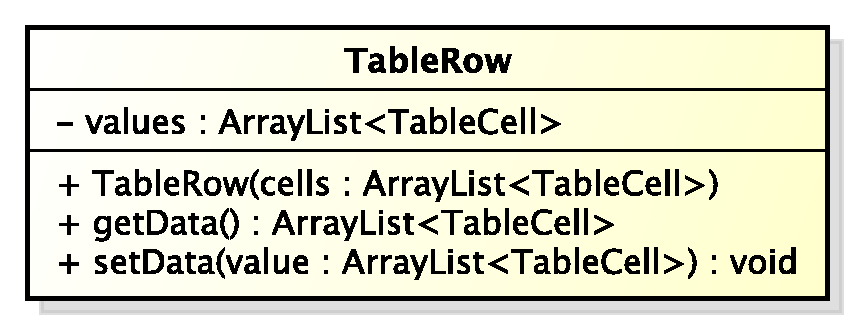
\includegraphics[scale=0.5]{DefinizioneDiProdotto/Pics/ClassiAggiuntive/TableRow}
				\caption{TableRow}
			\end{figure}
		}
	
			
			\begin{itemize}
			\item \textbf{Nome:} TableRow
			\item \textbf{Tipo:} classe
			
		\item \textbf{Astratta:}
		no
			\item \textbf{Visibilità:} public
			\item \textbf{Descrizione:} Tale classe rappresenta i dati di una riga di una table.
			\item \textbf{Attributi:}
				\begin{itemize}
				\setlength{\itemsep}{5pt}
				
					\item[\ding{111}] {--values : ArrayList<TableCell>} \\ [1mm] Tale attributo rappresenta i valori di una riga della table.
				\end{itemize}
		
			\item \textbf{Metodi:}
				\begin{itemize}
				\setlength{\itemsep}{5pt}
				
					\item[\ding{111}] {{+TableRow(cells : ArrayList<TableCell>)}} \\ [1mm] Tale metodo è il costruttore di TableRow. Esso ha come parametro i valori dei dati delle celle della riga della tabella.
					\item[\ding{111}] {{+getData() : ArrayList<TableCell>}} \\ [1mm] Tale metodo ha il compito di ritornare i dati della riga.
					\item[\ding{111}] {{+setData(value : ArrayList<TableCell>) : void}} \\ [1mm] Tale metodo ha il compito di impostare i dati della riga.
				\end{itemize}
		
			\end{itemize}
	
			\level{4}[TableSettingsImpl]{ApplicazioneAggiuntive::TableSettingsImpl}
			

		\IfFileExists{DefinizioneDiProdotto/Pics/ClassiAggiuntive/TableSettingsImpl.pdf}{
			\begin{figure}[H]
				\centering
				\includegraphics[scale=0.5]{DefinizioneDiProdotto/Pics/ClassiAggiuntive/TableSettingsImpl}
				\caption{TableSettingsImpl}
			\end{figure}
		}
	
			
			\begin{itemize}
			\item \textbf{Nome:} TableSettingsImpl
			\item \textbf{Tipo:} classe
			
		\item \textbf{Astratta:}
		no
			\item \textbf{Visibilità:} public
			\item \textbf{Descrizione:} Tale classe rappresenta le impostazioni di una table.
			\item \textbf{Attributi:}
				\begin{itemize}
				\setlength{\itemsep}{5pt}
				
					\item[\ding{111}] {--settings : JSONObject} \\ [1mm] Tale attributo memorizza l'Oggetto JSON con le impostazioni del chart.
				\end{itemize}
		
			\item \textbf{Metodi:}
				\begin{itemize}
				\setlength{\itemsep}{5pt}
				
					\item[\ding{111}] {{+TableSettingsImpl(settings : JSONObject)}} \\ [1mm] Tale metodo è il costruttore della classe. Esso ha il compito di creare l'oggetto e di inizializzarne i campi.
					\item[\ding{111}] {{+getCellBorderLineVisibility() : boolean}} \\ [1mm] Tale metodo ha il compito di ritornare un booleano che dica se lenee dei bordi delle celle devono esser visibili o no.
					\item[\ding{111}] {{+getTitle() : String}} \\ [1mm] Tale metodo ha il compito di ritornare il titolo del chart.
					\item[\ding{111}] {{+getDescription() : String}} \\ [1mm] Tale metodo ha il compito di ritornare la descrizione del chart.
					\item[\ding{111}] {{+getMaxValue() : String}} \\ [1mm] Tale metodo ha il compito di ritornare il numero massimo di valori consentiti nel chart.
				\end{itemize}
		
			\end{itemize}
	
			\level{4}[TableStreamUpdate]{ApplicazioneAggiuntive::TableStreamUpdate}
			

		\IfFileExists{DefinizioneDiProdotto/Pics/ClassiAggiuntive/TableStreamUpdate.pdf}{
			\begin{figure}[H]
				\centering
				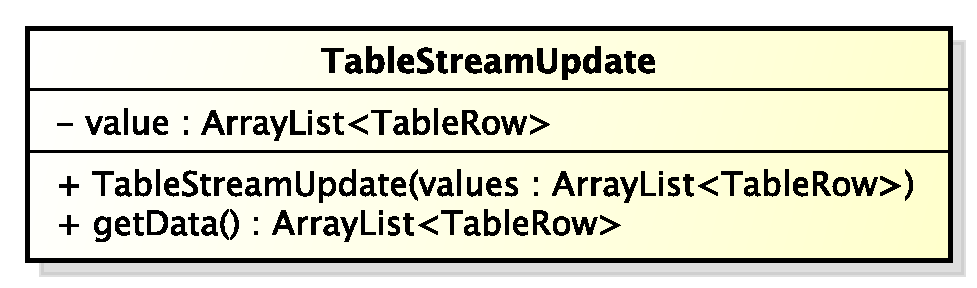
\includegraphics[scale=0.5]{DefinizioneDiProdotto/Pics/ClassiAggiuntive/TableStreamUpdate}
				\caption{TableStreamUpdate}
			\end{figure}
		}
	
			
			\begin{itemize}
			\item \textbf{Nome:} TableStreamUpdate
			\item \textbf{Tipo:} classe
			
		\item \textbf{Astratta:}
		no
			\item \textbf{Visibilità:} public
			\item \textbf{Descrizione:} Tale classe rappresenta un pacchetto di aggiornamento stream di una table.
			\item \textbf{Attributi:}
				\begin{itemize}
				\setlength{\itemsep}{5pt}
				
					\item[\ding{111}] {--value : ArrayList<TableRow>} \\ [1mm] Tale attributo rappresenta i valori del dato aggiornato.
				\end{itemize}
		
			\item \textbf{Metodi:}
				\begin{itemize}
				\setlength{\itemsep}{5pt}
				
					\item[\ding{111}] {{+TableStreamUpdate(values : ArrayList<TableRow>)}} \\ [1mm] Tale metodo è il costruttore per create tale pacchetto di aggiornamento.
					\item[\ding{111}] {{+getData() : ArrayList<TableRow>}} \\ [1mm] Tale metodo ha il compito di ritornare i nuovi dati del pacchetto di aggiornamento
				\end{itemize}
		
			\end{itemize}
	